% Section: forgetting curves beyond the exponential (input from main.tex)

\subsection{Why another curve}

The paper's recency term looks only at the last access and halves every 138 hours. Memory research describes forgetting differently. \citet{anderson1991reflections} measured how often an item comes back in natural environments (newspaper headlines, speech to children, electronic mail) and found that the probability of needing it again falls as a power of the time since each earlier occurrence and grows with the number of occurrences. Human retention follows the same power law \citep{wixted1991form}. ACT-R turns this into the base-level activation of a memory, $B_i=\ln\sum_j (T-t_{ij})^{-d}$ with $d=0.5$, a sum over every past use \citep{anderson2004integrated}. Agent memories have started to borrow such curves. MemoryBank strengthens a memory each time it is recalled \citep{zhong2024memorybank} and FadeMem decays memories with a stretched exponential \citep{wei2026fademem}. These systems say little about how to search a large memory under such a score, and the time-decayed vector search of \citet{wei2026tango} handles a single exponential of a fixed creation time.

This section uses the score
\begin{equation}
\mathrm{score}_i = a\,\widehat{D}_i + b\,\widehat{\imp}_i + c\,\widehat{\rel}_i,\qquad
D_i(T)=\sum_j \varphi(T-t_{ij}),\qquad \varphi(\Delta)=\Bigl(1+\frac{\Delta}{h_0}\Bigr)^{-d},
\label{eq:curvescore}
\end{equation}
where $t_{i1}<t_{i2}<\dots$ are the times at which memory $i$ was created or retrieved, $d=0.5$ as in ACT-R and $h_0=1$ hour keeps the curve finite at age zero. The hats are min-max scaling as before and $a=b=c=1$. This is ACT-R's sum without the logarithm, which cannot be folded (\cref{sec:curvelimits}). A second variant keeps only the last use, $D_i=\varphi(T-t_i)$, so that the curve is the only change from the paper.

\subsection{Any such curve is an inner product}

The power law, the hyperbolic curve $1/(1+\Delta/h)$ and stretched exponentials $e^{-\lambda\Delta^\beta}$ with $\beta\le1$ are completely monotone. By Bernstein's theorem every such function is a mixture of exponentials, $\varphi(\Delta)=\int e^{-\lambda\Delta}\,d\mu(\lambda)$ with $\mu\ge0$ \citep{widder1941laplace}, and a few terms of the mixture approximate it closely over any bounded range of ages \citep{beylkin2005expsums}:
\begin{equation}
\varphi(\Delta)\;\approx\;\varphi_R(\Delta)=\sum_{r=1}^{R} w_r\,e^{-\lambda_r\Delta},\qquad w_r\ge0 .
\end{equation}
The rates are spaced geometrically and the weights are fitted by non-negative least squares, with every error divided by the value of the curve, floored at 1\% of its start (\code{agentmem/curves.py}). \Cref{tab:curvefit} shows that the error shrinks quickly with $R$: eight exponentials follow ACT-R's curve over a whole year with an error of at most \CfActrRngEight{} of its range.

\begin{table}[t]
\centering\small
\begin{tabular}{r rr rr rr}
\toprule
 & \multicolumn{2}{c}{ACT-R} & \multicolumn{2}{c}{hyperbolic} & \multicolumn{2}{c}{FadeMem}\\
\cmidrule(lr){2-3}\cmidrule(lr){4-5}\cmidrule(lr){6-7}
$R$ & of range & relative & of range & relative & of range & relative\\
\midrule
4 & 5.82\% & 10.65\% & 3.00\% & 6.83\% & 2.76\% & 6.86\%\\
6 & 2.58\% & 3.47\% & 0.47\% & 1.01\% & 1.23\% & 2.24\%\\
8 & 0.30\% & 0.59\% & 0.06\% & 0.16\% & 0.36\% & 0.65\%\\
10 & 0.10\% & 0.14\% & 0.01\% & 0.03\% & 0.59\% & 0.62\%\\
12 & 0.02\% & 0.04\% & 0.00\% & 0.01\% & 0.20\% & 0.27\%\\
\bottomrule
\end{tabular}

\caption{Largest error of a sum of $R$ exponentials over ages from 0 to one year, as a share of the curve's range and relative to the curve where it is above 1\% of its start. ACT-R: $(1+\Delta/1\,\mathrm{h})^{-0.5}$. Hyperbolic: $1/(1+\Delta/24\,\mathrm{h})$. FadeMem: $e^{-0.1\,t^{0.8}}$ with $t$ in days, the long-term setting of \citet{wei2026fademem}.}
\label{tab:curvefit}
\end{table}

Every term of $\varphi_R$ factorises around an anchor $\tau$ as in \cref{eq:fold}, so
\begin{equation}
D^R_i(T)=\sum_{r=1}^{R} e^{-\lambda_r(T-\tau)}\;w_r\sum_j e^{-\lambda_r(\tau-t_{ij})}=\langle g(T),\,z_i(\tau)\rangle ,
\end{equation}
and with $x_i=[\,e_i;\ s\,z_i;\ s\,\imp_i\,]$ and $Q=[\,c\,q;\ (a/s)\,g(T);\ b/s\,]$ the score with the fitted curve is again $\langle Q,x_i\rangle$, now over $d+R+1$ dimensions. A memory does not need its whole history. It keeps $y_{ir}=\sum_j e^{-\lambda_r(t_i-t_{ij})}$ and its last use $t_i$, from which $z_{ir}(\tau)=w_r\,y_{ir}\,e^{-\lambda_r(\tau-t_i)}$, and a new use at time $t$ updates $y_{ir}\leftarrow y_{ir}\,e^{-\lambda_r(t-t_i)}+1$ in $O(R)$. Frequency therefore costs nothing extra. The paper's score is the case $R=1$ with $y_i\equiv1$.

The fit and the index are separate approximations. If $|\varphi_R-\varphi|\le\varepsilon\,\varphi$ on the ages that occur, then $|D^R_i-D_i|\le\varepsilon D_i$ for every memory, and when the fitted score of every memory is within $\eta$ of its true score, every memory in the fitted top-$k$ has a true score within $2\eta$ of the true $k$-th best. In the benchmark below an exact scan with the fitted curve returns \CuFitRecallOneM{} of the true top-10.

\subsection{A store for any curve}

The fitted rates span several orders of magnitude: for ACT-R's curve with $R=8$ the fastest is \CfFastRate{} per hour. The coordinate $e^{-\lambda_r(\tau-t_i)}$ of a memory used after the anchor grows by that factor every hour, so the hot segment of \cref{sec:fold}, anchored when it opens and filled for a week, no longer works. The store for general curves (\code{CurveFolded} in \code{agentmem/curve\_stores.py}) changes the order of events instead.
\begin{itemize}
\item A memory stays in a \emph{recent part} while its last use is younger than $W$ hours. The recent part is scored by a linear scan.
\item After that it moves to the hot segment. A hot segment is open for $L\le W$ hours and is anchored at $\tau=T_{\mathrm{open}}+L-W$.
\item Closed segments are merged as before and re-anchored at their latest use.
\end{itemize}
A memory enters a segment only when $t_i<T-W\le\tau$, so every stored coordinate lies in $[0,\,w_r\,y_{ir}]$ and every query factor $e^{-\lambda_r(T-\tau)}$ in $(0,1]$, for every rate, however fast. A retrieval moves the memories it returns back to the recent part, as the write buffer did before. The defaults are $W=L=24$ hours.

The normalisation needs the range of $D$. For a query factor with positive entries, $\max_i\langle g,z_i\rangle$ is reached on the Pareto-maximal set of the stored $z_i$ (those not dominated in every coordinate by another) and the minimum on the Pareto-minimal set, so the range of $D$ needs no search. The fronts are small: of the \CuSegN{} memories in the largest segment of the 100\,000-memory benchmark, \CuFrontMax{} are Pareto-maximal and \CuFrontMin{} Pareto-minimal. Deleting a memory that is not on a front leaves the fronts unchanged. The relevance range is estimated with the two searches for $\pm q$ as before, and small segments are simply scanned.

\subsection{Results}

\textbf{Retrieval at scale.} The benchmark of \cref{sec:static} is repeated with the score of \cref{eq:curvescore}. Every memory gets a use history: it is created at a uniform time over 90 days and used again a geometric number of times (1.2 on average) at uniform times after its creation. \Cref{tab:curvesstatic,fig:curves} show the results. An exact scan with the fitted curve returns \CuFitRecallOneM{} of the true top-10 with one million memories, so the fit itself costs almost nothing. The folded store returns \CuOursRecallHundredK{} of it with 100\,000 memories in \CuOursMsHundredK{} ms and \CuOursRecallOneM{} with one million in \CuOursMsOneM{} ms ($ef=64$). Overfetch returns \CuRerankOneM{} with $K=100$ and \CuRerankKOneM{} with $K=1000$, although it is given the exact normalisation ranges. Relevance only returns \CuRelOneM{}.

With one million memories most of the query time goes into the scan of the recent part, which in this history holds the \CuRecentOneM{} memories used in the last 24 hours. A recent part of 6 hours holds \CuRecentSixOneM{} memories and answers in \CuOursSixMsOneM{} ms, with recall \CuOursSixRecallOneM{}. More exponentials help up to a point: on 100\,000 memories at $ef=128$ recall is \CuRFour{}, \CuRSix{}, \CuREight{} and \CuRTen{} for $R=4$, 6, 8 and 10. As with the paper's score, part of the remaining loss comes from the estimated relevance range: with exact ranges the store reaches \CuRangeExact{} instead of \CuRangeEst{} on 100\,000 memories. The exact scan in this code takes \CuFitMsOneM{} ms per query on one million memories because it evaluates eight exponentials for every memory. Even a bare matrix-vector product, the least an exact scan can cost, takes about \GlExactMvMsOneM{} ms (\cref{sec:static}).

The curve changes what is retrieved. On the same one million memories, only \CuOverlapOneM{} of the top-10 under the ACT-R score are also in the top-10 under the paper's score (\CuOverlapHundredK{} with 100\,000 memories). Which curve suits an agent is a modelling question that this report does not answer. The point is that the index no longer constrains the answer.

\begin{table}[t]
\centering\small
\begin{tabular}{l rr rr}
\toprule
 & \multicolumn{2}{c}{100\,000 memories} & \multicolumn{2}{c}{1\,000\,000 memories}\\
\cmidrule(lr){2-3}\cmidrule(lr){4-5}
Method & recall@10 & ms & recall@10 & ms\\
\midrule
Exact scan, fitted curve ($R{=}8$) & 0.999 & 17 & 0.996 & 268\\
Folded HNSW, $ef{=}64$ (ours) & 0.982 & 0.70 & 0.969 & 2.40\\
Folded HNSW, $ef{=}256$ (ours) & 0.989 & 1.05 & 0.975 & 2.87\\
Folded HNSW, $ef{=}64$, $W{=}6$\,h (ours) & -- & -- & 0.954 & 1.55\\
Overfetch + re-rank, $K{=}100$ & 0.085 & 0.57 & 0.030 & 0.48\\
Overfetch + re-rank, $K{=}1000$ & 0.438 & 2.05 & 0.101 & 2.77\\
Relevance only & 0.014 & -- & 0.008 & --\\
\bottomrule
\end{tabular}

\caption{Recall@10 under the ACT-R score of \cref{eq:curvescore} (min-max, $a=b=c=1$, every use counted) on GloVe memories with synthetic use histories, and median query time. The folded store uses $R=8$ and a recent part of $W=24$ hours unless stated. Overfetch is given the exact normalisation ranges.}
\label{tab:curvesstatic}
\end{table}

\begin{figure}[t]
\centering
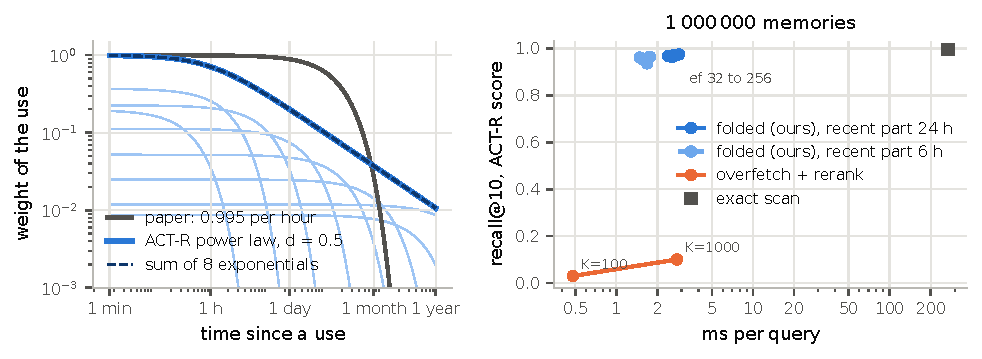
\includegraphics[width=0.99\linewidth]{curves}
\caption{Left: the weight of one use as a function of its age, for the paper's exponential and ACT-R's power law, with the eight exponentials (thin lines) whose sum (dashed) follows the power law. Right: recall@10 under the ACT-R score against query time with one million memories. Points along the folded curves are search depths, along overfetch candidate counts.}
\label{fig:curves}
\end{figure}

\subsection{Agents with a forgetting curve}
\label{sec:curvestown}

The party scenario of \cref{sec:town} was run again in the 32-day and 92-day runs, on the same 30 seeds, with ACT-R's curve in place of the paper's recency term. The curve takes two forms, of the last use only and summed over every use (\cref{eq:curvescore}). Each form is retrieved by an exact scan with the true curve, by the folded store ($R=8$, $W=L=24$ hours) and by overfetch and re-rank ($K=100$, with the newest memories added as in LangChain and exact normalisation ranges). In the town every segment is small enough for the folded store to compute its ranges by a scan. A third form takes ACT-R's logarithm of the sum. It cannot be folded and was run with the exact scan only. Recall is measured at every retrieval against the exact scan of the same score. \Cref{tab:curvestown} shows the outcomes.

\textbf{The folded store behaves like the exact scan with both foldable forms.} In the 92-day runs its retrievals contain \TcNinetyLastFoRecallFour{} of the true top-$k$ with the last use and \TcNinetyUsesFoRecallFour{} with every use. The three outcomes are identical on \TcNinetyLastFoSame{} and \TcNinetyUsesFoSame{} of the 30 seeds and differ by at most \TcNinetyUsesFoMaxDiff{} agents on the others. In the 32-day runs they are identical on \TcThirtyLastFoSame{} and \TcThirtyUsesFoSame{} seeds, with a largest difference of \TcThirtyUsesFoMaxDiff{} agents. At this memory size the exact scan is faster (\TcNinetyExMs{} against \TcNinetyFoMs{} ms per retrieval), as with the paper's score.

\textbf{The curve itself changes what the town does.} With exact retrieval and ACT-R's curve of the last use, \TcNinetyLastExAware{} agents know about the party at 92 days and \TcNinetyLastExRecalled{} recall it when planning, against \TcNinetyExpAware{} and \TcNinetyExpRecalled{} under the paper's exponential on the same seeds (paired Wilcoxon, Holm-adjusted $p=\TcNinetyLastVsExpAwareHolm{}$ and $p=\TcNinetyLastVsExpRecalledHolm{}$). In the 32-day runs the two curves give similar outcomes. The power law falls steeply in the first hours and slowly after that. After min-max scaling over 92 days, a memory last used five hours earlier keeps \TcShapeActrFive{} of the recency range under ACT-R's curve and \TcShapeExpFive{} under the exponential, one used 35 hours earlier \TcShapeActrThirtyFive{} and \TcShapeExpThirtyFive{}. Recency then mostly separates the last few hours from everything else, and among older memories importance weighs more. This probably helps the invitation, which is more important than most of what an agent observes.

\textbf{Counting every use locks the memory in.} With the sum over every use, only \TcNinetyUsesExRecalled{} agents recall the party when planning at 92 days and \TcNinetyUsesExAtt{} attend it, against \TcNinetyLastExRecalled{} and \TcNinetyLastExAtt{} with the last use (\TcThirtyUsesExRecalled{} against \TcThirtyLastExRecalled{} recalling it at 32 days). Every memory a retrieval returns counts as a use, so a memory that is retrieved gains weight and is retrieved again. Retrieval is concentrated under every form of the curve. At the end of \TcDiagSeeds{} of the 92-day runs, the 1\% most retrieved memories of an agent had received \TcDiagLastTopShare{} of its retrievals with the last use and \TcDiagUsesTopShare{} with every use. They are mostly pieces of news heard from other residents, which conversations bring up again and again. What differs is the effect on the score. With the last use a memory's recency term cannot exceed that of a fresh memory, so a memory heard an hour earlier still gets \TcDiagLastNewHour{} of the normalised range. Summed over every use, the most retrieved memories reach values of $D$ far above any single use, and the same memory gets \TcDiagUsesNewHour{}. ACT-R's logarithm compresses the range (\TcDiagLogNewHour{}) but changes the outcome little. With it the exact scan gives \TcNinetyLogExAware{} knowing agents, \TcNinetyLogExRecalled{} recalling the party and \TcNinetyLogExAtt{} guests. The lock-in therefore comes from counting retrievals as uses, not from leaving out the logarithm.

\textbf{Overfetch hides the problem.} With every use counted, overfetch returns only \TcNinetyUsesReRecall{} of the true top-$k$ at 92 days, yet \TcNinetyUsesReAware{} agents know about the party. Most of the memories that lock the score in probably never enter its candidate set, while the newest memories always do. Its outcome resembles the score of the last use more than the score it is meant to compute.

The index therefore no longer restricts the choice of curve, but the choice has to be tested in a closed loop. A score that looks reasonable on its own can lock an agent's memory in once every retrieval counts as a use.

\begin{table}[t]
\centering\small
\setlength{\tabcolsep}{4.5pt}
\begin{tabular}{l l l r r r r r}
\toprule
Run & Curve & Retrieval & memories & recall & knew & recalled & attended\\
\midrule
32 days & last use & Exact scan & 1736 & 1.000 & 12.1 $\pm$ 1.0 & 9.8 $\pm$ 1.1 & 5.1 $\pm$ 0.7\\
 &  & Folded HNSW (ours) & 1736 & 1.000 & 12.1 $\pm$ 1.0 & 9.8 $\pm$ 1.1 & 5.1 $\pm$ 0.7\\
 &  & Overfetch, $K{=}100$ & 1733 & 0.703 & 10.9 $\pm$ 1.0$^{**}$ & 9.1 $\pm$ 1.1$^{*}$ & 4.9 $\pm$ 0.6\\
\addlinespace[2pt]
 & every use & Exact scan & 1735 & 1.000 & 9.5 $\pm$ 1.0 & 5.8 $\pm$ 1.1 & 3.3 $\pm$ 0.6\\
 &  & Folded HNSW (ours) & 1735 & 1.000 & 9.3 $\pm$ 1.0 & 5.6 $\pm$ 1.0 & 3.2 $\pm$ 0.5\\
 &  & Overfetch, $K{=}100$ & 1734 & 0.601 & 10.9 $\pm$ 1.0$^{*}$ & 9.0 $\pm$ 1.1$^{**}$ & 4.8 $\pm$ 0.6$^{**}$\\
\addlinespace[2pt]
 & every use, log & Exact scan & 1736 & 1.000 & 10.0 $\pm$ 1.0 & 7.1 $\pm$ 1.0 & 3.9 $\pm$ 0.6\\
\addlinespace
92 days & last use & Exact scan & 5041 & 1.000 & 15.2 $\pm$ 1.4 & 12.4 $\pm$ 1.7 & 6.5 $\pm$ 1.0\\
 &  & Folded HNSW (ours) & 5041 & 1.000 & 15.1 $\pm$ 1.4 & 12.3 $\pm$ 1.7 & 6.4 $\pm$ 1.0\\
 &  & Overfetch, $K{=}100$ & 5033 & 0.536 & 15.2 $\pm$ 1.3 & 13.3 $\pm$ 1.3 & 6.8 $\pm$ 0.9\\
\addlinespace[2pt]
 & every use & Exact scan & 5034 & 1.000 & 9.2 $\pm$ 0.8 & 1.4 $\pm$ 0.2 & 1.2 $\pm$ 0.2\\
 &  & Folded HNSW (ours) & 5034 & 1.000 & 9.1 $\pm$ 0.8 & 1.4 $\pm$ 0.2 & 1.2 $\pm$ 0.2\\
 &  & Overfetch, $K{=}100$ & 5032 & 0.456 & 15.2 $\pm$ 1.3$^{**}$ & 11.5 $\pm$ 1.4$^{**}$ & 5.9 $\pm$ 0.9$^{**}$\\
\addlinespace[2pt]
 & every use, log & Exact scan & 5034 & 1.000 & 9.8 $\pm$ 1.0 & 2.8 $\pm$ 0.5 & 1.8 $\pm$ 0.3\\
\bottomrule
\end{tabular}

\caption{The party scenario with ACT-R's curve in place of the paper's recency term, of the last use, summed over every use and, with the exact scan only, the logarithm of that sum. Columns as in \cref{tab:town}. Recall is against the exact scan of the same score. Stars mark a difference from that exact scan in a paired Wilcoxon test, Holm-corrected over the 24 comparisons in the table ($^{*}p<0.05$, $^{**}p<0.01$).}
\label{tab:curvestown}
\end{table}

\subsection{Limits}
\label{sec:curvelimits}

\begin{itemize}
\item ACT-R takes the logarithm of the sum before adding other sources of activation. The logarithm does not change which of two memories has the larger recency-frequency term, but it changes how that term trades off against importance and relevance, and the logarithm of an inner product is not an inner product. The score used here keeps the sum, which favours frequently used memories more than ACT-R does. In the town the logarithm changes little (\cref{sec:curvestown}).
\item What locks the memory in is that every retrieved memory counts as a use. Remedies that still fold exist, for example a smaller weight for a retrieval than for the observation itself or a cap on the number of uses that count, but they are not tested here.
\item The curve's parameters are ACT-R's usual choices, not values fitted to agents, and the use histories of the scale test are synthetic.
\item Decay rates that differ from memory to memory, as in MemoryBank and FadeMem, fold only when they take a few values, with one block of coordinates per value. This is not implemented.
\item The recent part is scanned, so its cost grows with the number of memories used in the last $W$ hours. Compaction rebuilds the merged segment from scratch, which is cheap for one agent's memory but would need a tiered scheme for millions of memories.
\end{itemize}
